\section{Background Theory}
\label{sec:background_theory}
\subsection{Convolutional Neural Networks}
A \ac{CNN} is a special kind of neural network, and it was one of the first deep learning models to perform well in commercial applications. A \ac{CNN} is loosely based on principles drawn from neuroscience. According to \cite{Bengio_deep_learning_book},  local connectivity and parameter sharing are properties characteristic for \ac{CNN}s. These properties and the architecture of \ac{CNN}s will be explored further below.

\subsubsection{Convolution}
In mathematics, convolution is a mathematical operation on two real-valued functions that express the amount of overlap of one function as it is shifted over another function. For machine learning applications, the data is usually discretized. The operation is therefore a discrete summation over the data, and is used to calculate the weighted sum between the activations and the connection weights in a \ac{CNN}. The discrete convolution operation without kernel-flipping:

$$ (x*w)(t) = \sum\limits_{a=-\infty}^\infty x[a]w[t+a]$$ 

For aerial images we extend the convolution operation to two dimensions, and limit the summation to a finite number of pixels. To convolve an image I, a two-dimensional kernel K containing the weights is shifted across the image:  

$$ (I*K)[i,j] = \sum\limits_{m}\sum\limits_{n} I[i+m, j+n]K[m,n]$$ 

This operation is  visualized in figure \ref{fig:convolution} where a $2 \times 2$ kernel of weights is convolved with a $3 \times 3$ matrix of input values, and produces $2 \times 3$ outputs. 

\begin{figure}[t]
\begin{center}
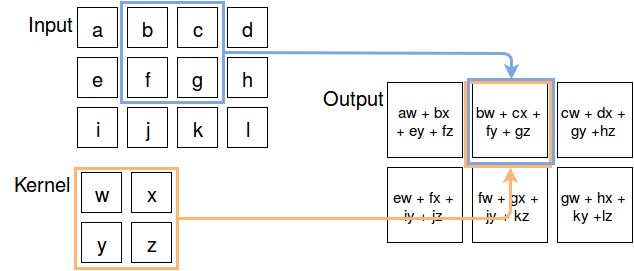
\includegraphics[width=0.8\columnwidth]{figs/convolution.png}
\caption[Convolution example]{Example of 2D convolution without kernel-flipping.}
\label{fig:convolution}
\end{center}
\end{figure}


\subsubsection{Local Connectivity}
In a traditional neural network, each layer is typically fully connected. Each unit has connections to every unit in the previous layer. In a \ac{CNN}, however, a unit interacts only with a small region of units in the previous layer. This region is often referred to as the unit's local receptive field. This kind of local connectivity can be very practical for high-dimensional data, such as images where meaningful features can be extracted using only a small area of the total image. \\

Local connectivity can be achieved by using a small kernel as seen in Figure \ref{fig:convolution}. Instead of each unit being connected to all inputs, the unit only depends on a $2 \times 2$ input region. \\

If there are $m$ inputs and $n$ units, a matrix multiplication for a fully-connected network would require $m\times n$ parameters, as well as having a runtime of $O(m\times n)$. By using a kernel we limit the number of connections each unit may have to k. This requires only $k\times n$ parameters and a runtime of $O(k\times n)$. For image applications, the kernel size can be relatively small and still achieve good results, which can give big improvements in efficiency.

\subsubsection{Parameter Sharing}
The number of model parameters is further reduced by using parameter sharing. Each weight in the kernel is applied to every position of the input. In contrast, a neural network which is fully connected will have a separate weight for every connection. This can be redundant for high-dimensional data, where most of the features are localized. In images, for example, an important feature to extract are edges. A kernel with weights that are good at detecting edges at one location, will be equally good at detecting them in other locations. \\

The use of parameter sharing further reduces the storage requirement to $k$ parameters. Usually, one kernel per layer is not enough, so several kernels with tied weights convolve the input. The layer will then produce output activations for different features. The outputs of several kernels are often referred to as feature maps.

\subsubsection{Pooling}
The pooling function is another operation typically associated with \ac{CNN}s. A pooling function modifies the output of a layer in some way. It replaces a rectangular region of the output by a single value that has been determined by a summary operation. A common pooling function is the max pooling operation, which outputs the maximum within a rectangular neighborhood. The reason for utilizing pooling is that it helps the representation become invariant to small translations in the input. For example, a network created to classify whether an image depicts a cat or not will benefit from pooling, since the location of the cat in the picture is irrelevant. For tasks where the location of a feature is important, such as semantic segmentation, applying pooling should be done with restraint. Additionally, pooling reduces the number of input parameters for the next layer.

\subsubsection{Layer Structure}
A typical convolutional layer in a network consists of three stages. First, convolution sums the weighted inputs for every unit in the layer. Second, an activation function is applied to the resulting values. The \ac{ReLU} is a popular choice, and outputs either 0 or the weighted sum, depending on which is biggest: $f(x) = max(0, x)$. Finally, the pooling function modifies the output of the layer. 

\subsubsection{Network architecture}
A \ac{CNN} usually consists of both convolutional layers and fully-connected layers. The input layer and the initial hidden layers are convolutional layers, with fully connected layers attached at the end. Figure \ref{fig:conv} shows a convolutional neural network configuration. The input layer and the two first hidden layers are convolutional layers. During training, the kernel weights for these layers are adjusted by backpropagation. Each feature map defines a set of kernel weights that are applied to all input pixels or activations. Usually, a \ac{CNN} will reduce the necessity of feature engineering because it learns what suitable features to extract from input data. In images, a \ac{CNN} is able to learn from raw pixel values without the use of feature extraction techniques found in computer vision.


\begin{figure}[t]
\begin{center}
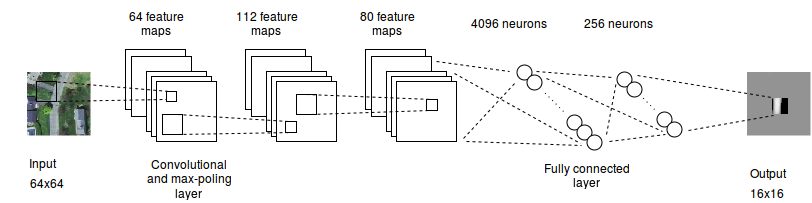
\includegraphics[width=1\columnwidth]{figs/conv_diagram.png}
\caption[Convolutional neural network]{Convolutional neural network. }
\label{fig:conv}
\end{center}
\end{figure}
\label{sec:convolutional_networks_background}

\subsection{Label Noise}
\label{sec:background_label_noise}
There are several reasons for the presence of inconsistent labels in real-world datasets. For instance, the labeller was presented with insufficient information, or the dataset was automatically generated from a source with poor quality labels. Additionally, the samples could be ambiguous and therefore hard to label correctly by a human expert. Label noise, can in many cases, lead to negative consequences for a classifier. This can include reduced accuracy, increased model complexity, and more samples required for learning a target concept. Approaches for dealing with noisy labels can generally be divided into three groups: Data cleansing methods, noise-robust models, and noise-tolerant algorithms \citep{Frenay_label_noise_survey}. These three groups are presented below.  \\

%\subsubsection{Types of noisy labels}
%Based on the noise distribution, three types of label noise can be identified according a extensive survey on label noise by \citep{Frenay_label_noise_survey}. The different types can be viewed in Figure ??\todo{Figur}. X is a vector of features or the data. For all types the observed variable Y* is assumed to depend the true label Y.  The E is a binary variable indicating if an labelling error has occurred. 

%Noisy completely at random (NCAR) model.

%Noisy at random (NAR) model. 

%Noisy not at random (NNAR) model


\subsubsection{Data Cleansing Methods}

Data cleansing methods are filtering techniques applied to the training data in order to remove noisy samples before training. Noisy labels are first identified and then either relabelled or removed. An obstacle encountered by these methods is that harmful mislabelled samples can be difficult to distinguish from informative, but hard samples. Another problem is that filtering often relies on classifier predictions to automatically identify mislabelled samples. Such filtering techniques also run the risk of removing too many samples from the training set, which can also cause harm to the accuracy. Voting ensembles of several classifiers have been suggested to further improve classification filtering.\\ 

Another filtering technique is to simply remove the class label of samples deemed suspicious, and employ semi-supervised learning. This way, the distribution of samples are preserved while simultaneously reducing the consequences of inconsistent labels.\\


\subsubsection{Noise-robust Models}
Noise-robust models are algorithms that are naturally robust against label noise. Many algorithms have been shown to be less sensitive to label noise than others, especially to small amounts of label noise. This approach requires no noise modelling nor cleansing of the training set beforehand, because the algorithm is assumed to offer some robustness to mislabelled samples.\\

 Algorithms that utilize regularization techniques to avoid overfitting, can be considered more robust to label noise. This can include convolutional networks that utilize regularization schemes such as dropout or weight decay. For ensemble methods, bagging often gives better results than boosting when faced with noisy labels \citep{Dietterich_boosting_bagging}. The boosting algorithm AdaBoost, for example, combines many weak classifiers by iteratively re-weighting the training set to target samples the previous classifier had trouble predicting. Because mislabelled samples can be harder to predict, AdaBoost tends to put larger emphasis on mislabelled samples in later stages of learning, which can lead to increased sensitivity to label noise. In bagging methods, however, different subsets of the training data are used to create a diverse set of classifiers that are employed in a voting scheme. In this case, mislabelled samples can impact the performance positively, due to the increased variability in the classifiers.   


\subsubsection{Noise-tolerant Algorithms}
In noise-tolerant approaches, existing algorithms are modified to be more robust towards label noise. This is often done by explicitly modelling a noise model during training. This way, a classifier learns to classify samples according to their true uncorrupted label, instead of the observed noisy label. Typically, the noise distribution and the model parameters are estimated simultaneously when training the classifier. \\

Techniques that incorporate label noise tolerance, such as particle competition, noise model estimation, bootstrapping, and co-training, will be further discussed in Section \ref{sec:related_works}.

\subsection{Curriculum Learning}
Curriculum learning is inspired by how humans learn, and that learning typically is highly organized. For instance, by the use of a curriculum in educational institutions. Easier concepts tend to be introduced first. In terms of machine learning, this means presenting the classifier with easier samples first while training. To do so, a curriculum strategy has to be defined, which sorts the training set from easy to hard. Samples that are not near the decision boundary could be considered easy, for instance. Utilizing curriculum learning might lead to a faster convergence time, and help the algorithm reach a better local minimum. Different works show that curriculum learning can achieve better generalization for many tasks \citep{Bengio_curriculumlearning} \citep{Kumar_self_paced_learning} \citep{Lu_self-paced_learning_diversity}.\\

A challenge for curriculum learning is defining a sorting measure that enables a curriculum strategy of gradually introducing harder training samples to the learner. This issue, and works related to curriculum learning, is further explored in Section \ref{sec:related_works}.\\

\subsection{Road Extraction by Machine Learning}
Road extraction is a part of the field of Photogrammetry, and involves technology for map production and measurements of objects in images. As digital acquisition systems for capturing aerial images have become commonplace, the availability of high-resolution aerial images have increased. Coupled with the increasing need for detailed spatial information in \ac{GIS} databases and production of digital maps, a lot of approaches for automatic object extraction from aerial imagery have been suggested. A reliable and accurate detection system could be beneficial in terms of increased levels of details, while reducing the cost associated with map production.\\

There are three distinctive approaches for extracting objects from aerial imagery. Manual, semi-automatic and automatic methods. The semi-automatic approach integrates computer vision techniques and machine learning into the workflow of skilled human labellers. For instance, Google's Ground Truth project employs skilled operators which utilize advanced software tools to improve the accuracy of Google's map products \citep{Ground_truth}.\\

To do automatic road detection, supervised learning is often employed. This requires a training dataset of aerial images and labels. The labels for road detection are usually binary images that show the ground truth of roads. Creating the label images by manually labelling aerial imagery would be prohibitively expensive, which is why ground truth labels are often generated from existing map data. Figure \ref{fig:background_dataset_example} shows an example of an aerial image and a label typically found in a road segmentation dataset.\\

\begin{figure}
\begin{subfigure}{0.40\textwidth}
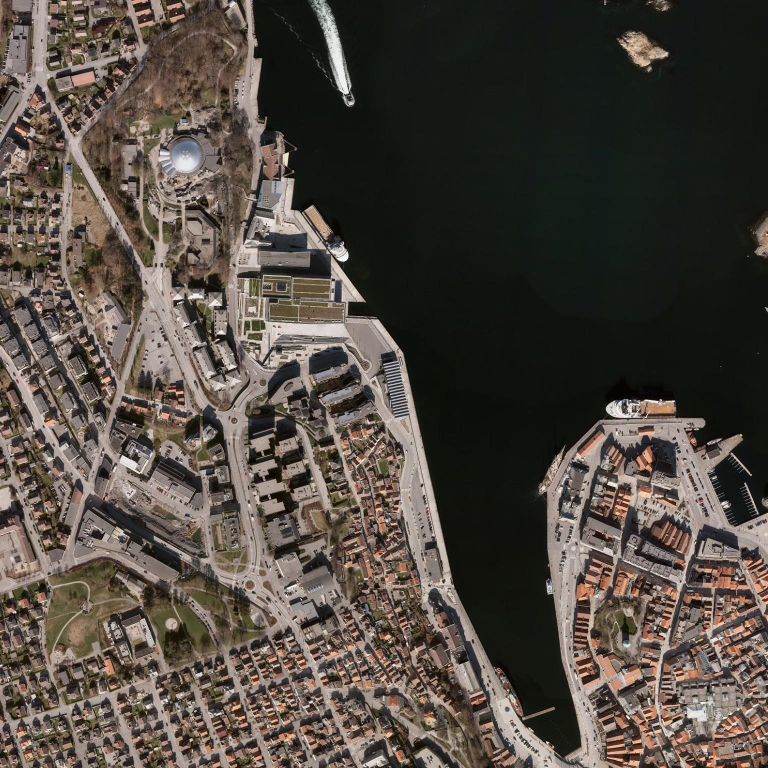
\includegraphics[width=\linewidth]{figs/background_theory_example_data.png}
\caption{Aerial image} \label{fig:background_dataset_example_data}
\end{subfigure}
\hspace*{\fill} % separation between the subfigures
\begin{subfigure}{0.40\textwidth}
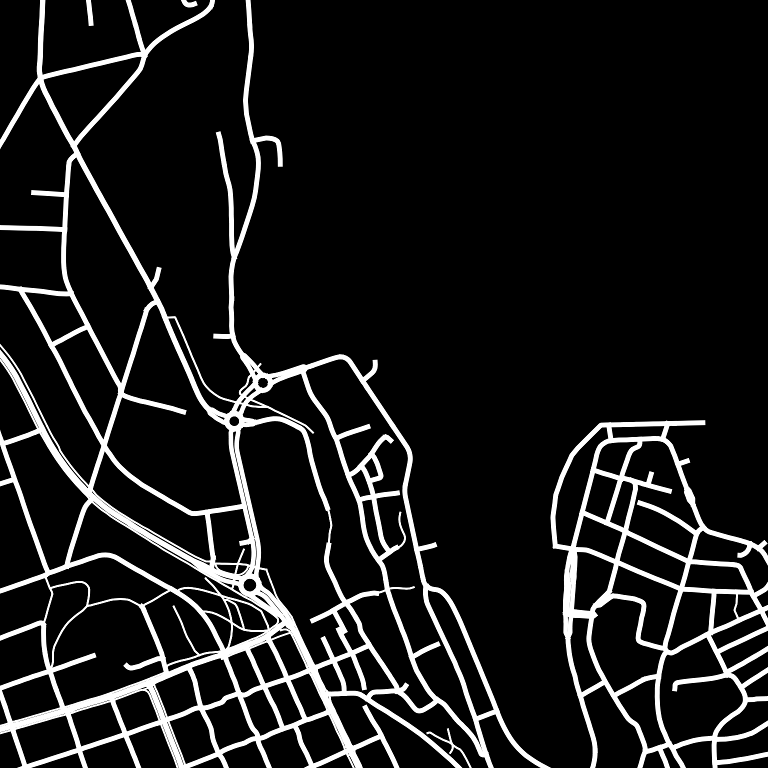
\includegraphics[width=\linewidth]{figs/background_theory_example_label.png}
\caption{Label image} \label{fig:background_dataset_example_label}
\end{subfigure}
\caption[Example from the Norwegian Roads Dataset]{Image and label example from the training set of the Norwegian Roads Dataset.} \label{fig:background_dataset_example}
\end{figure}

From these large training set images, smaller training set patches are extracted. The supervised learning algorithm is given a patch dataset $d$ containing $N$ training examples in the form $d=\{(s_1, m_1),...,(s_N, m_N)\}$, where $s_i$ is an aerial image patch and $m_i$ is the corresponding ground truth label. Examples of aerial image patches and labels can be found in Figure \ref{fig:examples_background}. The learning algorithm's task is to learn a suitable mapping from the input space of aerial imagery to the output space of road ground truth. In neural networks, this mapping is typically learned by minimizing the cross-entropy loss by gradient descent optimization.\\

\begin{figure}
\begin{center}
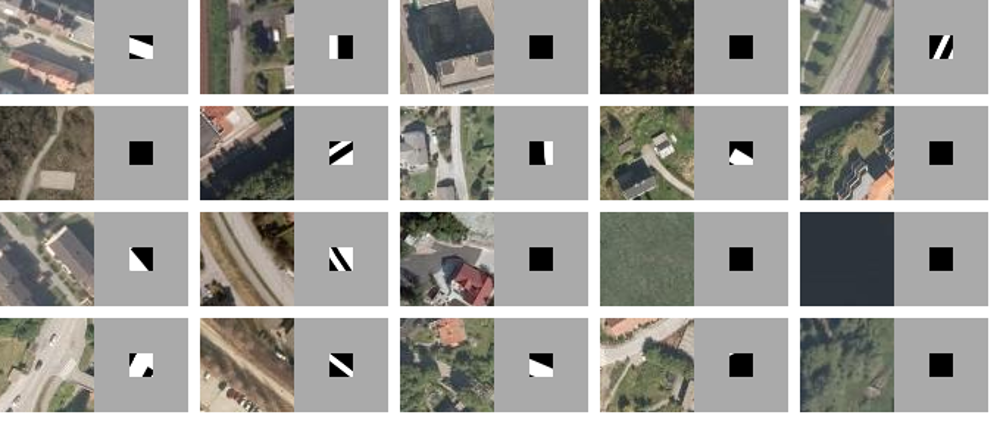
\includegraphics[width=1\columnwidth]{figs/examples.png}
\caption[Patch dataset examples]{Aerial image and label examples from a patch dataset. The patches originate from the Norwegian Roads Dataset. Each label depicts the road ground truth from the center location of the aerial patch.}
\label{fig:examples_background}
\end{center}
\end{figure}

 The resulting classifier has hopefully extracted some useful patterns from the training data, which enables it to generalize to the task of road extraction. This is verified by computing the \ac{MSE} on a test set, containing examples not seen during training. The machine learning approach for road extraction should therefore be able to train algorithms from data which can predict the ground truth reasonable well for new unseen aerial image patches. \\

\subsection{Evaluation Metrics}
A common way to evaluate road extraction systems is by the quality measures,  correctness and completeness \citep{Wiedemann_road_evaluation}. These are closely related to precision and recall. Precision measures the fraction of true roads that are correctly detected, while recall is the fraction of predicted roads that are true roads. Because the label maps are not perfectly aligned with the images, it is also common to use a relaxed measure of precision and recall. This is accomplished by treating predicted road pixels within $p$ pixels of a true road pixel as being correctly detected. True roads within $p$ pixels of a predicted road pixel are considered correctly recalled. The slack parameter $p$ is often set to 3 pixels \citep{Mnih_roads_high_res_aerial_images}.

